\documentclass{article}
\usepackage[polish]{babel}
\usepackage[T1]{fontenc}
\usepackage{geometry}
\usepackage{chngpage}
\usepackage{graphicx}
\usepackage{subcaption}
\usepackage{amsfonts}
\graphicspath{ {./plots/} }
\geometry{margin=2cm}
\usepackage[utf8]{inputenc}
\usepackage{indentfirst}
\usepackage{longtable}
\author{Nie interesuj się}
\title{Sprawozdanie}
\frenchspacing
\setlength{\parindent}{3em}
\begin{document}
\maketitle
\section*{Zadanie Pierwsze}
\noindent \textbf{Cel: } Zbadanie wpływu niewielkich zmian danych na końcowy wynik.\\\\
\noindent \textbf{Przebieg doświadczenia: } Badanie będzimy przeprowadzać na przerobionym już wcześnie przykładzie z listy pierwszej.  Doświadczenie przeprowadzone poprzednio polegało na obliczeniu iloczynu skalarnego dla dwóch zadanych wektorów \\\\
$A= [2.718281828, -3.141592654, 1.414213562, 0.5772156649, 0.3010299957]$ \\
$B= [1486.2497, 878366.9879, -22.37492, 4773714.647, 0.000185049]$\\\\
\noindent Tym razem zminiejszymy dokładność, poprzez pozbycie się liczb znaczących w $A_{4}$ (pozbywamy się najmniejszej cyfry części ułamkowej - '9'), oraz $A_{5}$ (pozbywamy się ostatniej cyfry części ułamkowej - '7'). Po dokonaniu obliczeń porównamy je z poprzednimi wynikami.\\\\
Poprzednim razem badania przeprowadzaliśmy dla czterech różnych algorytmów, tym razem także je wykorzystamy, są to:
\begin{enumerate}
	\item Algorytm 1 (``w przód'') - przejście wprost po wektorze, sumując kolejne wyrazy, zaczynając od początku tablicy
	\item Algorytm 2 (``w tył'') - przejście wprost po wektorze, sumując kolejne wyrazy, zaczynając od końca tablicy
	\item Algorytm 3 (``od najmniejszego do największego'') - posortowanie iloczynów rosnąco a następnie dodanie ich po kolei do dwóch akumulatorów, jeden dla liczb dodatnich, drugi dla liczb ujemnych a ostatecznie zsumowanie obu akumulatorów.
	\item Algorytm 4 (``od największego do najmniejszego'') - posortowanie iloczynów malejąco a następnie dodanie ich po kolei do dwóch akumulatorów, jeden dla liczb dodatnich, drugi dla liczb ujemnych a ostatecznie zsumowanie obu akumulatorów.\\\\
\end{enumerate}
\noindent \textbf{Wyniki:} \\\\Poprzednio otrzymane wyniki przedstawiają się następująco:
\begin{center}
	\begin{tabular}{|p{2,5cm}|p{3cm}|p{5cm}|} \hline
		\textbf{Algorytm} & \textbf{Float32} & \textbf{Float64} \\
		\hline
		\textbf{1} & $-0.4999443$ & $1.0251881368296672*10^{-10}$ \\
		\hline
		\textbf{2} & $-0.4543457$ & $-1.5643308870494366*10^{-10}$ \\
		\hline
		\textbf{3} & $-0.5$ & $0.0$  \\
		\hline
		\textbf{4} & $-0.5$ & $0.0$ \\
		\hline
	\end{tabular}
\end{center}

\noindent Aktualne wyniki po usunięciu w/w cyfr:
\begin{center}
	\begin{tabular}{|p{2,5cm}|p{3cm}|p{5cm}|} \hline
		\textbf{Algorytm} & \textbf{Float32} & \textbf{Float64} \\
		\hline
		\textbf{1} & $-0.4999443$ & $-0.004296342739891585$ \\
		\hline
		\textbf{2} & $-0.4543457$ & $-0.004296342998713953$ \\
		\hline
		\textbf{3} & $-0.5$ & $-0.004296342842280865$ \\
		\hline
		\textbf{4} & $-0.5$ & $-0.004296342842280865$ \\
		\hline
	\end{tabular}
\end{center}

\noindent \textbf{Wnioski:} \\\\
W przypadku Float32, zmiana nie miała wpływu na wynik ze względu na zbyt małą precyzję obliczeń. W przypadku dwukrotnego zwiększenia dokładności (Float64), otrzymaliśmy dużą różnicę w wynikach. Nie otrzymaliśmy już zer, a wyniki poszczególnych algorytmów są teraz do siebie zbliżone. Zmiana rzędu $10^{-9}$ spowodowała zmiejszenie ortogonalności (prostopadłości) wektora. To zadanie jest przykładem zadania źle uwarunkowanego, w którym niewielka zmiana danych powoduje olbrzymie zmiany w wynikach. W tym przypadku jest to spowodowane prostopadłością wektorów.
\section*{Zadanie Drugie}
\noindent \textbf{Cel: } Porównanie wykresów funkcji $f(x)$ z obliczoną granicą tejże funkcji.\\\\
\noindent \textbf{Funkcja: } 
$$ f(x) = e^{x}*ln(1+e^{-x}) $$\\
\noindent \textbf{Obliczona pochodna: }
$$\lim_{x \to \infty} e^{x}*ln(1+e^{-x}) = \lim_{x \to \infty} \frac{ln(1+e^{-x})}{e^{-x}}  \stackrel{de'hospital}{=} \lim_{x \to \infty} \frac{1}{1+e^{-x}} = 1  $$
\noindent \textbf{Wykresy: }
\begin{figure}[ht]
	\begin{subfigure}{.5\textwidth}
	\centering
	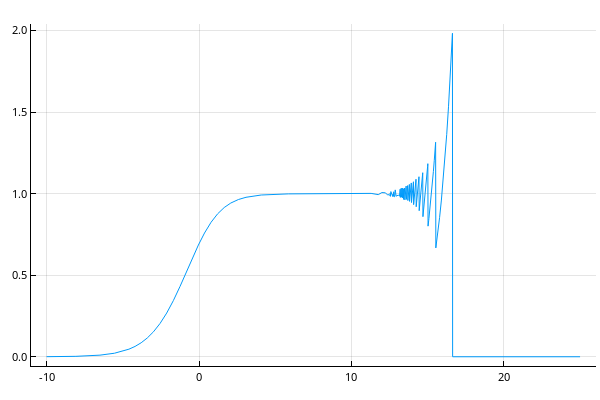
\includegraphics[width=.8\linewidth]{JuliaPlots/Float32(-10-25)}  
	\caption*{Float32, zakres [-10,25]}

\end{subfigure}
\begin{subfigure}{.5\textwidth}
	\centering
	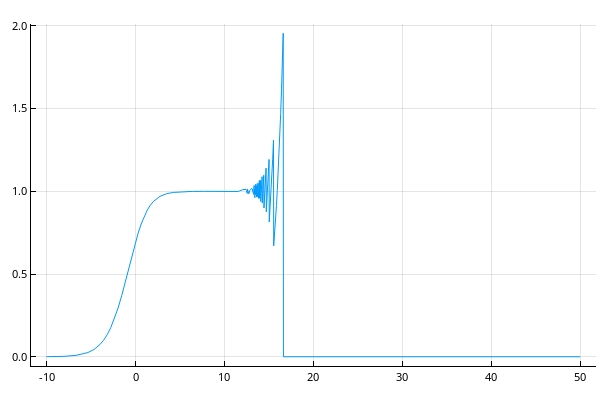
\includegraphics[width=.8\linewidth]{JuliaPlots/Float32(-10-50)}  
	\caption*{Float32, zakres [-10,50]}

	\end{subfigure}
\end{figure}
\begin{figure}[ht]
	\begin{subfigure}{.5\textwidth}
		\centering
		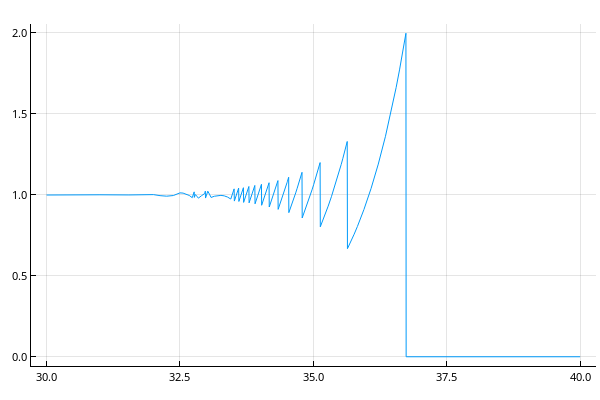
\includegraphics[width=.8\linewidth]{JuliaPlots/Float64(30-40)}  
		\caption*{Float64, zakres [30,40]}

	\end{subfigure}
	\begin{subfigure}{.5\textwidth}
		\centering
		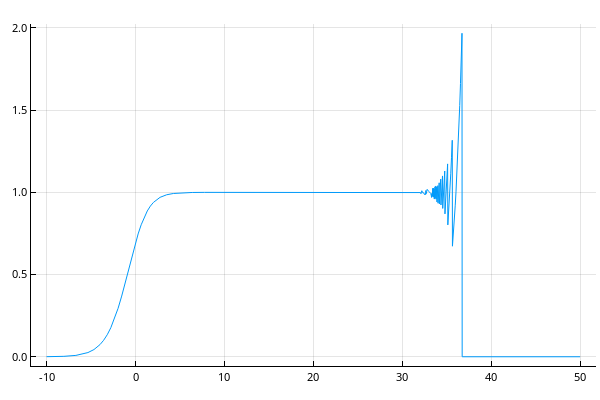
\includegraphics[width=.8\linewidth]{JuliaPlots/Float64(-10-50)}  
		\caption*{Float64, zakres [-10,50]}

	\end{subfigure}
\end{figure}
\begin{figure}[ht]
	\begin{subfigure}{.5\textwidth}
		\centering
		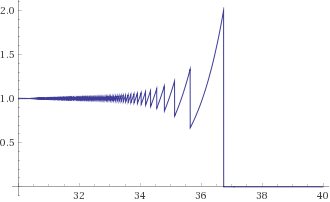
\includegraphics[width=.8\linewidth]{WolfPlots/Screenshot_2019-11-06 f(x) = (((exp(x)) ((log((1) + (exp(-x))))))) for x range(30,40) - Wolfram Alpha}  
		\caption*{WolframAlpha, zakres [30,40]}

	\end{subfigure}
	\begin{subfigure}{.5\textwidth}
		\centering
		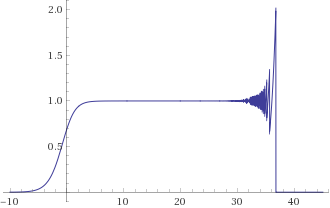
\includegraphics[width=.8\linewidth]{WolfPlots/Screenshot_2019-11-06 f(x) = (((exp(x)) ((log((1) + (exp(-x))))))) for x range(-10,45) - Wolfram Alpha}  
		\caption*{WolframAlpha, zakres [-10,45]}

	\end{subfigure}
\end{figure} \\
\newpage
\noindent \textbf{Wnioski:} \\\\
Otrzymane wykresy różnią się w znacznym stopniu od oczekiwanego rezultatu. Oczekiwany wykres miał być zbieżny do jedynki, podczas gdy na otrzymanych wykresach widoczne są zaburzenia. Jest to spowodowane pochłanianiem małych wartości $e^{-x} $ przez jedynkę. Dodatkowo, w momencie w którym $ 1 + e^{-x} = 1 $ ($e^{-x} = 0$ dla zadanej precyzji) to $ln(1 + e^{-x}) = 0$. \\\\ Bardzo ciekawy wypadek zauważa się w przypadku użycia wolframalpha, bo po pewnym momencie zwraca on „nagle” poprawny wynik:\\
\begin{figure}[ht]
	\begin{subfigure}{.5\textwidth}
		\centering
		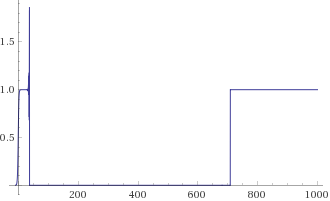
\includegraphics[width=.8\linewidth]{WolfPlots/Screenshot_2019-11-06 f(x) = (((exp(x)) ((log((1) + (exp(-x))))))) for x range(-10,1000) - Wolfram Alpha}  
		\caption*{WolframAlpha, zakres [-10,1000]}

	\end{subfigure}
\end{figure} \\
Może być to spowodowane faktem iż wolfram posiada wiele sposobów obliczania pochodnych, więc kiedy kończy mu się zakres zmiennej, przechodzi na inną metodę, która podaje już dobry wynik.

\section*{Zadanie Trzecie}
\noindent \textbf{Cel: } Rozwiązanie układu równań liniowych\\\\
\noindent \textbf{Funkcja: }
$$ Ax =b $$ 
gdzie:\\
$A$ - macierz, taka że $A \in \mathbb{R}^{n \times n}$\\
$b$ - wektor prawych stron $\textbf{b} \in \mathbb{R}^{n}$ \\\\
\newpage
\noindent \textbf{Wyniki:} \\\\
Dla macierzy Hilberta:
\begin{center}
	\begin{tabular}{|p{1cm}|p{1cm}|p{4cm}|p{4cm}|p{4cm}|} \hline
		\textbf{n} & \textbf{rząd} & \textbf{wskaźnik \newline uwarunkowania} & \textbf{błąd Gaussa} & \textbf{błąd macierzy \newline odwrotnej}  \\
		\hline
		$1$ & $1$ & $1.0$ & $0.0$ & $0.0$  \\
		\hline
		$2$ & $2$ & $19.28147006790397$ & $4.227603326225575e-16$ & $1.4043333874306803e-15$  \\
		\hline
		$3$ & $3$ & $524.0567775860644$ & $6.312995352117186e-16$ & $0.0$  \\
		\hline
		$4$ & $4$ & $15513.73873892924$ & $2.1819484005185015e-15$ & $4.547473508864641e-13$  \\
		\hline
		$5$ & $5$ & $476607.25024259434$ & $8.99737540851766e-12$ & $1.4911297558868156e-11$  \\
		\hline
		$6$ & $6$ & $1.4951058642254665e7$ & $1.8866554820446764e-10$ & $3.5689314550268525e-10$  \\
		\hline
		$7$ & $7$ & $4.75367356583129e8$ & $1.8614175017153493e-8$ & $1.231617281152939e-8$  \\
		\hline
		$8$ & $8$ & $1.5257575538060041e10$ & $1.9217530132542664e-7$ & $1.3503856270597747e-7$  \\
		\hline
		$9$ & $9$ & $4.931537564468762e11$ & $5.09208671414057e-6$ & $9.542631496737485e-6$  \\
		\hline
		$10$ & $10$ & $1.6024416992541715e13$ & $5.508778842434553e-5$ & $0.0002289249459044258$  \\
		\hline
		$11$ & $10$ & $5.222677939280335e14$ & $0.005207147400142043$ & $0.008849600746399502$  \\
		\hline
		$12$ & $10$ & $1.7514731907091464e16$ & $0.1407902677571603$ & $0.4039460424541017$  \\
		\hline
		$13$ & $11$ & $3.344143497338461e18$ & $355.6363996139929$ & $212.78257870436312$  \\
		\hline
		$14$ & $11$ & $6.200786263161444e17$ & $3.5720053119125916$ & $1.7744875020766255$  \\
		\hline
		$15$ & $11$ & $3.674392953467974e17$ & $9.583022643862336$ & $5.293638550842115$  \\
		\hline
		$16$ & $12$ & $7.865467778431645e17$ & $11.968066192267113$ & $10.846229140698135$  \\
		\hline
		$17$ & $12$ & $1.263684342666052e18$ & $5.455797564762254$ & $8.982730231514317$  \\
		\hline
		$18$ & $12$ & $2.2446309929189128e18$ & $26.309523680963647$ & $20.038300611698062$  \\
		\hline
		$19$ & $13$ & $6.471953976541591e18$ & $22.59171398621913$ & $15.359549749376397$  \\
		\hline
		$20$ & $13$ & $1.3553657908688225e18$ & $5.658540758579833$ & $7.992554067235351$  \\
		\hline
	\end{tabular}
\end{center}
Dla macierzy losowej:
\begin{center}
	\begin{tabular}{|p{1cm}|p{1cm}|p{4cm}|p{4cm}|p{4cm}|} \hline
		\textbf{n} & \textbf{rząd} & \textbf{wskaźnik \newline uwarunkowania} & \textbf{błąd Gaussa} & \textbf{błąd macierzy \newline odwrotnej}  \\
		\hline
		$5$ & $5$ & $1.0000000000000002$ & $2.895107444979072e-16$ & $2.531698018113677e-16$  \\
		\hline
		$5$ & $5$ & $10.000000000000012$ & $3.2934537262255424e-16$ & $2.808666774861361e-16$  \\
		\hline
		$5$ & $5$ & $999.9999999999957$ & $2.9918399161602327e-15$ & $8.407255028117242e-15$  \\
		\hline
		$5$ & $5$ & $9.999999998272197e6$ & $6.098113193176361e-10$ & $4.920721043551264e-10$  \\
		\hline
		$5$ & $5$ & $1.0000569317412089e12$ & $2.090745266471979e-5$ & $2.2491352852287535e-5$  \\
		\hline
		$5$ & $4$ & $6.163423754077854e15$ & $0.2055523184662983$ & $0.059292706128157104$  \\
		\hline
		$10$ & $10$ & $1.0000000000000007$ & $1.7901808365247238e-16$ & $1.6088660122137096e-16$  \\
		\hline
		$10$ & $10$ & $9.999999999999996$ & $2.1355566272775288e-16$ & $2.603703785810335e-16$  \\
		\hline
		$10$ & $10$ & $999.9999999999403$ & $9.215519889170636e-16$ & $3.640448215221993e-15$  \\
		\hline
		$10$ & $10$ & $1.0000000004304033e7$ & $1.1869428686627522e-11$ & $5.182444144318803e-11$  \\
		\hline
		$10$ & $10$ & $1.0000237542007422e12$ & $3.68036568648752e-5$ & $3.532974000347535e-5$  \\
		\hline
		$10$ & $9$ & $8.183587485979556e15$ & $0.11886587922969834$ & $0.12082884330738251$  \\
		\hline
		$20$ & $20$ & $1.0000000000000016$ & $4.0867669957713655e-16$ & $4.6510262453954645e-16$  \\
		\hline
		$20$ & $20$ & $9.999999999999988$ & $5.822058658345461e-16$ & $4.6510262453954645e-16$  \\
		\hline
		$20$ & $20$ & $1000.0000000000192$ & $2.7950391086350172e-14$ & $2.958989099482218e-14$  \\
		\hline
		$20$ & $20$ & $1.0000000002579732e7$ & $6.232949674212794e-11$ & $9.084754966320824e-11$  \\
		\hline
		$20$ & $20$ & $1.0000894285296765e12$ & $2.633880965470748e-5$ & $2.4529436866417026e-5$  \\
		\hline
		$20$ & $19$ & $9.36557482791752e15$ & $0.3098253119813586$ & $0.30186113977303886$  \\
		\hline
	\end{tabular}
\end{center}
\newpage
\noindent \textbf{Wnioski:} \\\\
Patrząc na wyniki otrzymane z obliczeń dla macierzy losowej możemy stwierdzić, że potwierdzają one wpływ wskaźnika uwarunkowania macierzy na wielkość błędu względnego. Są one proporcjonalne, tj. jeżeli rośnie wskaźnik uwarunkowania, rośnie także błąd względny. Każdy problem o dużym wskaźniku uwarunkowania nazywamy problemem źle uwarunkowanym.\\\\
Przykładem problemu źle uwarukowanego jest analizowana przez nas macierz Hilberta - wraz ze wzrostem wielkości macierzy rośnie także współczynnik uwarunkowania. Dodatkowo, z analizy wyników można wywnioskować że metoda Gaussa jest skuteczniejsza przy wyliczaniu błędu względnego dla macierzy Hilberta.
\section*{Zadanie Czwarte}
\noindent \textbf{Cel:} Obliczyć 20 miejsc zerowych wielomianu $p$ Wilkinsona ($p(x) = (x-20)(x-19)...(x-2)(x-1)$) w postaci naturalnej i sprawdzenie poprawności (błędu otrzymanych pierwiastków) a następnie doświadczenie powtórzyć zmieniając $(-210)*x^{19} \rightarrow (-210-2^{-23})*x^{19}$, w zapisie binarnym zmiana wygląda nastepująco:
$$ (-210) \rightarrow  11000000011010100100000000000000000000000\textbf{0}0000000000000000000000$$
$$ (-210-2^{-23}) \rightarrow 11000000011010100100000000000000000000000\textbf{1}0000000000000000000000$$
\noindent \textbf{Wyniki:} \\\\
Dla macierzy Wilkinsona przed zaburzeniem:
\begin{center}
	\begin{tabular}{|p{0,3cm}|p{3,5cm}|p{3,5cm}|p{3,5cm}|p{4cm}|} \hline
		\textbf{k} & \textbf{$z_{k}$} & \textbf{$|P(z_{k})|$} & \textbf{$|p(z_{k})$} & \textbf{$|z_{k} - k$}  \\
		\hline 
		$1$ & $0.9999999999996989$ & $36352.0$ & $38400.0$ & $3.0109248427834245e-13$ \\ 
		\hline 
		$2$ & $2.0000000000283182$ & $181760.0$ & $198144.0$ & $2.8318236644508943e-11$ \\ 
		\hline 
		$3$ & $2.9999999995920965$ & $209408.0$ & $301568.0$ & $4.0790348876384996e-10$ \\ 
		\hline 
		$4$ & $3.9999999837375317$ & $3.106816e6$ & $2.844672e6$ & $1.626246826091915e-8$ \\ 
		\hline 
		$5$ & $5.000000665769791$ & $2.4114688e7$ & $2.3346688e7$ & $6.657697912970661e-7$ \\ 
		\hline 
		$6$ & $5.999989245824773$ & $1.20152064e8$ & $1.1882496e8$ & $1.0754175226779239e-5$ \\ 
		\hline 
		$7$ & $7.000102002793008$ & $4.80398336e8$ & $4.78290944e8$ & $0.00010200279300764947$ \\ 
		\hline 
		$8$ & $7.999355829607762$ & $1.682691072e9$ & $1.67849728e9$ & $0.0006441703922384079$ \\ 
		\hline 
		$9$ & $9.002915294362053$ & $4.465326592e9$ & $4.457859584e9$ & $0.002915294362052734$ \\ 
		\hline 
		$10$ & $9.990413042481725$ & $1.2707126784e10$ & $1.2696907264e10$ & $0.009586957518274986$ \\ 
		\hline 
		$11$ & $11.025022932909318$ & $3.5759895552e10$ & $3.5743469056e10$ & $0.025022932909317674$ \\ 
		\hline 
		$12$ & $11.953283253846857$ & $7.216771584e10$ & $7.2146650624e10$ & $0.04671674615314281$ \\ 
		\hline 
		$13$ & $13.07431403244734$ & $2.15723629056e11$ & $2.15696330752e11$ & $0.07431403244734014$ \\ 
		\hline 
		$14$ & $13.914755591802127$ & $3.65383250944e11$ & $3.653447936e11$ & $0.08524440819787316$ \\ 
		\hline 
		$15$ & $15.075493799699476$ & $6.13987753472e11$ & $6.13938415616e11$ & $0.07549379969947623$ \\ 
		\hline 
		$16$ & $15.946286716607972$ & $1.555027751936e12$ & $1.554961097216e12$ & $0.05371328339202819$ \\ 
		\hline 
		$17$ & $17.025427146237412$ & $3.777623778304e12$ & $3.777532946944e12$ & $0.025427146237412046$ \\ 
		\hline 
		$18$ & $17.99092135271648$ & $7.199554861056e12$ & $7.1994474752e12$ & $0.009078647283519814$ \\ 
		\hline 
		$19$ & $19.00190981829944$ & $1.0278376162816e13$ & $1.0278235656704e13$ & $0.0019098182994383706$ \\ 
		\hline 
		$20$ & $19.999809291236637$ & $2.7462952745472e13$ & $2.7462788907008e13$ & $0.00019070876336257925$ \\ 
		\hline 
	\end{tabular}
\end{center}
\newpage
\noindent Dla macierzy Wilkinsona po zaburzeniu
\begin{center}
	\begin{tabular}{|p{0,3cm}|p{3,5cm}|p{3,5cm}|p{3,5cm}|p{4cm}|} \hline
		\textbf{k} & \textbf{$z_{k}$} & \textbf{$|P(z_{k})|$} & \textbf{$|p(z_{k})$} & \textbf{$|z_{k} - k$}  \\
		\hline 
		$1$ & $0.9999999999998357$ & $20992.0$ & $22016.0$ & $1.6431300764452317e-13$ \\ 
		\hline 
		$2$ & $2.0000000000550373$ & $349184.0$ & $365568.0$ & $5.503730804434781e-11$ \\ 
		\hline 
		$3$ & $2.99999999660342$ & $2.221568e6$ & $2.295296e6$ & $3.3965799062229962e-9$ \\ 
		\hline 
		$4$ & $4.000000089724362$ & $1.046784e7$ & $1.0729984e7$ & $8.972436216225788e-8$ \\ 
		\hline 
		$5$ & $4.99999857388791$ & $3.9463936e7$ & $4.3303936e7$ & $1.4261120897529622e-6$ \\ 
		\hline 
		$6$ & $6.000020476673031$ & $1.29148416e8$ & $2.06120448e8$ & $2.0476673030955794e-5$ \\ 
		\hline 
		$7$ & $6.99960207042242$ & $3.88123136e8$ & $1.757670912e9$ & $0.00039792957757978087$ \\ 
		\hline 
		$8$ & $8.007772029099446$ & $1.072547328e9$ & $1.8525486592e10$ & $0.007772029099445632$ \\ 
		\hline 
		$9$ & $8.915816367932559$ & $3.065575424e9$ & $1.37174317056e11$ & $0.0841836320674414$ \\ 
		\hline 
		$10$ & $10.095455630535774$ & $7.143113638035824e9$ & $1.4912633816754019e12$ & $0.6519586830380406$ \\ 
		\hline 
		$11$ & $10.095455630535774$ & $7.143113638035824e9$ & $1.4912633816754019e12$ & $1.1109180272716561$ \\ 
		\hline 
		$12$ & $11.793890586174369$ & $3.357756113171857e10$ & $3.2960214141301664e13$ & $1.665281290598479$ \\ 
		\hline 
		$13$ & $11.793890586174369$ & $3.357756113171857e10$ & $3.2960214141301664e13$ & $2.045820276678428$ \\ 
		\hline 
		$14$ & $13.992406684487216$ & $1.0612064533081976e11$ & $9.545941595183662e14$ & $2.5188358711909045$ \\ 
		\hline 
		$15$ & $13.992406684487216$ & $1.0612064533081976e11$ & $9.545941595183662e14$ & $2.7128805312847097$ \\ 
		\hline 
		$16$ & $16.73074487979267$ & $3.315103475981763e11$ & $2.7420894016764064e16$ & $2.9060018735375106$ \\ 
		\hline 
		$17$ & $16.73074487979267$ & $3.315103475981763e11$ & $2.7420894016764064e16$ & $2.825483521349608$ \\ 
		\hline 
		$18$ & $19.5024423688181$ & $9.539424609817828e12$ & $4.2525024879934694e17$ & $2.454021446312976$ \\ 
		\hline 
		$19$ & $19.5024423688181$ & $9.539424609817828e12$ & $4.2525024879934694e17$ & $2.004329444309949$ \\ 
		\hline 
		$20$ & $20.84691021519479$ & $1.114453504512e13$ & $1.3743733197249713e18$ & $0.8469102151947894$ \\ 
		\hline 
	\end{tabular}
\end{center}
\noindent \textbf{Wnioski:} \\\\
Jak widać nawet minimalne odchylenie przekształca w bardzo duży wynik końcowy. W tym wielomianie zamiast zer otrzymujemy wyniki rzędu bilionów. Natomiast drobna zmiana powoduje ogromne różnice w wynikach między dwoma wielomianami (w obu nie uzyskujemy zer). To przypadek źle uwarunkowanego zadania. Warto 
pamiętać, że wyniki zależą od ilości cyfr znaczących w przypadku arytmetyki Float64 wynosi ona od 15 do 17 cyfr znaczących.
\section*{Zadanie Piąte}
\noindent \textbf{Cel:} Badanie modelu wzrostu populacji $p_{n}$\\\\
\noindent \textbf{Wzór rekurencyjny:}
$$p_{n+1} = p_{n} + r*p_{n}*(1-p_{n})$$
gdzie: \\
$r$ - dana stała \\
$p_{0}$ - wielkość populacji stanowiąca procent maksymalnej wielkości populacji dla danego stanu środowiska.\\\\
\newpage
\noindent \textbf{Wyniki:} \\\\
Dla obciętego wyniku (zmodyfikowana rekurencja) w 10 iteracji, oraz normalna rekurencja (Float32):
\begin{center}
	\begin{tabular}{|p{0,3cm}|p{5cm}|p{5cm}|} \hline
		\textbf{n} & \textbf{czysta rekurencja} & \textbf{zmodyfikowana rekurencja}  \\
		\hline 
		$1$ & $0.0397$ & $0.0397$ \\ 
		\hline
		$2$ & $0.15407173$ & $0.15407173$ \\ 
		\hline
		$3$ & $0.5450726$ & $0.5450726$ \\ 
		\hline
		$4$ & $1.2889781$ & $1.2889781$ \\ 
		\hline
		$5$ & $0.1715188$ & $0.1715188$ \\ 
		\hline
		$6$ & $0.5978191$ & $0.5978191$ \\ 
		\hline
		$7$ & $1.3191134$ & $1.3191134$ \\ 
		\hline
		$8$ & $0.056273222$ & $0.056273222$ \\ 
		\hline
		$9$ & $0.21559286$ & $0.21559286$ \\ 
		\hline
		$10$ & $0.7229306$ & $0.722$ \\ 
		\hline
		$11$ & $1.3238364$ & $1.3241479$ \\ 
		\hline
		$12$ & $0.037716985$ & $0.036488414$ \\ 
		\hline
		$13$ & $0.14660022$ & $0.14195944$ \\ 
		\hline
		$14$ & $0.521926$ & $0.50738037$ \\ 
		\hline
		$15$ & $1.2704837$ & $1.2572169$ \\ 
		\hline
		$16$ & $0.2395482$ & $0.28708452$ \\ 
		\hline
		$17$ & $0.7860428$ & $0.9010855$ \\ 
		\hline
		$18$ & $1.2905813$ & $1.1684768$ \\ 
		\hline
		$19$ & $0.16552472$ & $0.577893$ \\ 
		\hline
		$20$ & $0.5799036$ & $1.3096911$ \\ 
		\hline
		$21$ & $1.3107498$ & $0.09289217$ \\ 
		\hline
		$22$ & $0.088804245$ & $0.34568182$ \\ 
		\hline
		$23$ & $0.3315584$ & $1.0242395$ \\ 
		\hline
		$24$ & $0.9964407$ & $0.94975823$ \\ 
		\hline
		$25$ & $1.0070806$ & $1.0929108$ \\ 
		\hline
		$26$ & $0.9856885$ & $0.7882812$ \\ 
		\hline
		$27$ & $1.0280086$ & $1.2889631$ \\ 
		\hline
		$28$ & $0.9416294$ & $0.17157483$ \\ 
		\hline
		$29$ & $1.1065198$ & $0.59798557$ \\ 
		\hline
		$30$ & $0.7529209$ & $1.3191822$ \\ 
		\hline
		$31$ & $1.3110139$ & $0.05600393$ \\ 
		\hline
		$32$ & $0.0877831$ & $0.21460639$ \\ 
		\hline
		$33$ & $0.3280148$ & $0.7202578$ \\ 
		\hline
		$34$ & $0.9892781$ & $1.3247173$ \\ 
		\hline
		$35$ & $1.021099$ & $0.034241438$ \\ 
		\hline
		$36$ & $0.95646656$ & $0.13344833$ \\ 
		\hline
		$37$ & $1.0813814$ & $0.48036796$ \\ 
		\hline
		$38$ & $0.81736827$ & $1.2292118$ \\ 
		\hline
		$39$ & $1.2652004$ & $0.3839622$ \\ 
		\hline
		$40$ & $0.25860548$ & $1.093568$ \\ 
		\hline
	\end{tabular}
\end{center}
\newpage
Porównawcze wyniki dla Float32 i Float64:
\begin{center}
	\begin{tabular}{|p{0,3cm}|p{5cm}|p{5cm}|} \hline
		\textbf{n} & \textbf{Float32} & \textbf{Float64}  \\
		\hline 
		$1$ & $0.0397$ & $0.0397$ \\ 
		\hline
		$2$ & $0.15407173$ & $0.15407173000000002$ \\ 
		\hline
		$3$ & $0.5450726$ & $0.5450726260444213$ \\ 
		\hline
		$4$ & $1.2889781$ & $1.2889780011888006$ \\ 
		\hline
		$5$ & $0.1715188$ & $0.17151914210917552$ \\ 
		\hline
		$6$ & $0.5978191$ & $0.5978201201070994$ \\ 
		\hline
		$7$ & $1.3191134$ & $1.3191137924137974$ \\ 
		\hline
		$8$ & $0.056273222$ & $0.056271577646256565$ \\ 
		\hline
		$9$ & $0.21559286$ & $0.21558683923263022$ \\ 
		\hline
		$10$ & $0.7229306$ & $0.722914301179573$ \\ 
		\hline
		$11$ & $1.3238364$ & $1.3238419441684408$ \\ 
		\hline
		$12$ & $0.037716985$ & $0.03769529725473175$ \\ 
		\hline
		$13$ & $0.14660022$ & $0.14651838271355924$ \\ 
		\hline
		$14$ & $0.521926$ & $0.521670621435246$ \\ 
		\hline
		$15$ & $1.2704837$ & $1.2702617739350768$ \\ 
		\hline
		$16$ & $0.2395482$ & $0.24035217277824272$ \\ 
		\hline
		$17$ & $0.7860428$ & $0.7881011902353041$ \\ 
		\hline
		$18$ & $1.2905813$ & $1.2890943027903075$ \\ 
		\hline
		$19$ & $0.16552472$ & $0.17108484670194324$ \\ 
		\hline
		$20$ & $0.5799036$ & $0.5965293124946907$ \\ 
		\hline
		$21$ & $1.3107498$ & $1.3185755879825978$ \\ 
		\hline
		$22$ & $0.088804245$ & $0.058377608259430724$ \\ 
		\hline
		$23$ & $0.3315584$ & $0.22328659759944824$ \\ 
		\hline
		$24$ & $0.9964407$ & $0.7435756763951792$ \\ 
		\hline
		$25$ & $1.0070806$ & $1.315588346001072$ \\ 
		\hline
		$26$ & $0.9856885$ & $0.07003529560277899$ \\ 
		\hline
		$27$ & $1.0280086$ & $0.26542635452061003$ \\ 
		\hline
		$28$ & $0.9416294$ & $0.8503519690601384$ \\ 
		\hline
		$29$ & $1.1065198$ & $1.2321124623871897$ \\ 
		\hline
		$30$ & $0.7529209$ & $0.37414648963928676$ \\ 
		\hline
		$31$ & $1.3110139$ & $1.0766291714289444$ \\ 
		\hline
		$32$ & $0.0877831$ & $0.8291255674004515$ \\ 
		\hline
		$33$ & $0.3280148$ & $1.2541546500504441$ \\ 
		\hline
		$34$ & $0.9892781$ & $0.29790694147232066$ \\ 
		\hline
		$35$ & $1.021099$ & $0.9253821285571046$ \\ 
		\hline
		$36$ & $0.95646656$ & $1.1325322626697856$ \\ 
		\hline
		$37$ & $1.0813814$ & $0.6822410727153098$ \\ 
		\hline
		$38$ & $0.81736827$ & $1.3326056469620293$ \\ 
		\hline
		$39$ & $1.2652004$ & $0.0029091569028512065$ \\ 
		\hline
		$40$ & $0.25860548$ & $0.011611238029748606$ \\ 
		\hline
	\end{tabular}
\end{center}
\newpage
\noindent \textbf{Wykresy:} \\\\
\begin{figure}[ht]
	\begin{subfigure}{.5\textwidth}
		\centering
		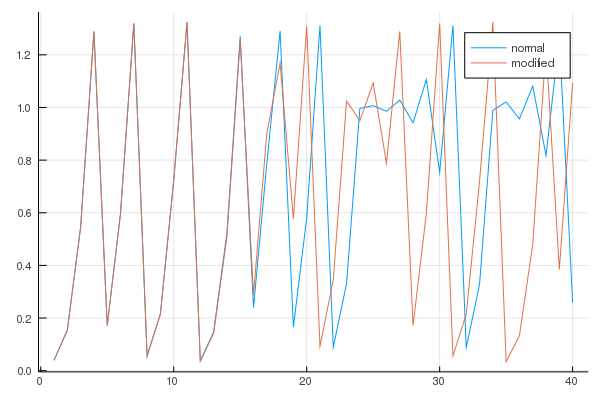
\includegraphics[width=.8\linewidth]{JuliaPlots/comparition1}  
		\caption*{Porównanie graficzne (tabela pierwsza)}
		
	\end{subfigure}
	\begin{subfigure}{.5\textwidth}
		\centering
		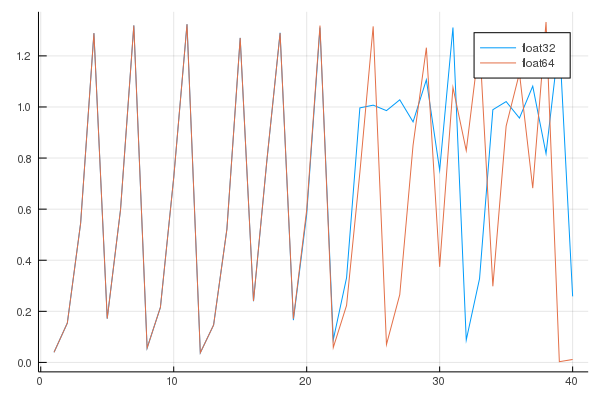
\includegraphics[width=.8\linewidth]{JuliaPlots/comparition2}  
		\caption*{Porównanie graficzne (tabela druga)}
		
	\end{subfigure}
\end{figure}\\
\begin{figure}[ht]
\centering
	\begin{subfigure}{.5\textwidth}
		\centering
		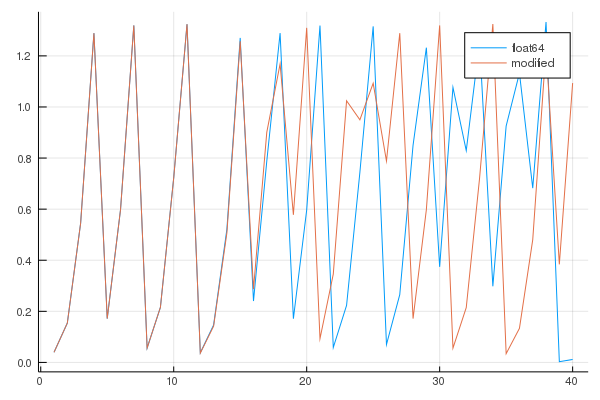
\includegraphics[width=.8\linewidth]{JuliaPlots/comparition3}  
		\caption*{Porównanie graficzne float64 z ucietą rekurencją}
		
	\end{subfigure}
\end{figure}\\
\noindent \textbf{Wnioski:} \\\\
Widzimy, że wykonane przez nas ekperymenty mają związek ze sprzężeniem zwrotnym (dane wyjściowe przekładają się na dane wejściowe do następnego obliczenia z serii obliczeń). Oznacza to że nawt mała zmiana na początku ciągu obliczeń może powodować olbrzymie odchylenia w dalszych iteracjach. Ponadto widzimy punkt   załamania  w którym dana arytmetyka traci swoją precyzję i od tego punktu $x$ dane bedą zaszumione. Główna różnica między trzema wynikami (obcięty float32, float32 i float64) jest położenie tego punktu na osi (0,x), które rośnie wraz z precyzją arytmetyki.
\section*{Zadanie Szóste}
\noindent \textbf{Cel:} Badanie równanie rekurencyjnego\\\\
\noindent \textbf{Wzór:}
$$x_{n+1} = x^{2}_{n} +c, dla \, n = 0,1...$$
\newpage
\noindent \textbf{Wyniki:}\\\\
Dla $c = -2$:
\begin{center}
	\begin{tabular}{|p{2cm}|p{2cm}|p{2cm}|p{3,8cm}| } \hline
		\textbf{$iteracja$} & \textbf{$x_{0}=1$} & \textbf{$x_{0}=2$} & \textbf{$x_{0}=1.99999999999999$}  \\
		\hline
		$1$ & $-1$ & $2$ & $1.99999999999996$  \\ 
		\hline
		$2$ & $-1$ & $2$ & $1.9999999999998401$  \\ 
		\hline
		$3$ & $-1$ & $2$ & $1.9999999999993605$  \\ 
		\hline
		$4$ & $-1$ & $2$ & $1.999999999997442$  \\ 
		\hline
		$5$ & $-1$ & $2$ & $1.9999999999897682$  \\ 
		\hline
		$6$ & $-1$ & $2$ & $1.9999999999590727$  \\ 
		\hline
		$7$ & $-1$ & $2$ & $1.999999999836291$  \\ 
		\hline
		$8$ & $-1$ & $2$ & $1.9999999993451638$  \\ 
		\hline
		$9$ & $-1$ & $2$ & $1.9999999973806553$  \\ 
		\hline
		$10$ & $-1$ & $2$ & $1.999999989522621$  \\ 
		\hline
		$11$ & $-1$ & $2$ & $1.9999999580904841$  \\ 
		\hline
		$12$ & $-1$ & $2$ & $1.9999998323619383$  \\ 
		\hline
		$13$ & $-1$ & $2$ & $1.9999993294477814$  \\ 
		\hline
		$14$ & $-1$ & $2$ & $1.9999973177915749$  \\ 
		\hline
		$15$ & $-1$ & $2$ & $1.9999892711734937$  \\ 
		\hline
		$16$ & $-1$ & $2$ & $1.9999570848090826$  \\ 
		\hline
		$17$ & $-1$ & $2$ & $1.999828341078044$  \\ 
		\hline
		$18$ & $-1$ & $2$ & $1.9993133937789613$  \\ 
		\hline
		$19$ & $-1$ & $2$ & $1.9972540465439481$  \\ 
		\hline
		$20$ & $-1$ & $2$ & $1.9890237264361752$  \\ 
		\hline
		$21$ & $-1$ & $2$ & $1.9562153843260486$  \\ 
		\hline
		$22$ & $-1$ & $2$ & $1.82677862987391$  \\ 
		\hline
		$23$ & $-1$ & $2$ & $1.3371201625639997$  \\ 
		\hline
		$24$ & $-1$ & $2$ & $-0.21210967086482313$  \\ 
		\hline
		$25$ & $-1$ & $2$ & $-1.9550094875256163$  \\ 
		\hline
		$26$ & $-1$ & $2$ & $1.822062096315173$  \\ 
		\hline
		$27$ & $-1$ & $2$ & $1.319910282828443$  \\ 
		\hline
		$28$ & $-1$ & $2$ & $-0.2578368452837396$  \\ 
		\hline
		$29$ & $-1$ & $2$ & $-1.9335201612141288$  \\ 
		\hline
		$30$ & $-1$ & $2$ & $1.7385002138215109$  \\ 
		\hline
		$31$ & $-1$ & $2$ & $1.0223829934574389$  \\ 
		\hline
		$32$ & $-1$ & $2$ & $-0.9547330146890065$  \\ 
		\hline
		$33$ & $-1$ & $2$ & $-1.0884848706628412$  \\ 
		\hline
		$34$ & $-1$ & $2$ & $-0.8152006863380978$  \\ 
		\hline
		$35$ & $-1$ & $2$ & $-1.3354478409938944$  \\ 
		\hline
		$36$ & $-1$ & $2$ & $-0.21657906398474625$  \\ 
		\hline
		$37$ & $-1$ & $2$ & $-1.953093509043491$  \\ 
		\hline
		$38$ & $-1$ & $2$ & $1.8145742550678174$  \\ 
		\hline
		$39$ & $-1$ & $2$ & $1.2926797271549244$  \\ 
		\hline
		$40$ & $-1$ & $2$ & $-0.3289791230026702$  \\ 
		\hline
	\end{tabular}
\end{center}
\newpage
Dla $c = -1$:
\begin{center}
	\begin{tabular}{|p{1,5cm}|p{1,5cm}|p{1,5cm}|p{4,5cm}|p{4,5cm}| } \hline
		\textbf{$iteracja$} & \textbf{$x_{0}=1$} & \textbf{$x_{0}=-1$} & \textbf{$x_{0}=0.75$} & \textbf{$x_{0}=0.25$}  \\
		\hline
		$1$ & $0$ & $0$ & $-0.4375$ & $-0.9375$ \\ 
		\hline
		$2$ & $-1$ & $-1$ & $-0.80859375$ & $-0.12109375$ \\ 
		\hline
		$3$ & $0$ & $0$ & $-0.3461761474609375$ & $-0.9853363037109375$ \\ 
		\hline
		$4$ & $-1$ & $-1$ & $-0.8801620749291033$ & $-0.029112368589267135$ \\ 
		\hline
		$5$ & $0$ & $0$ & $-0.2253147218564956$ & $-0.9991524699951226$ \\ 
		\hline
		$6$ & $-1$ & $-1$ & $-0.9492332761147301$ & $-0.0016943417026455965$ \\ 
		\hline
		$7$ & $0$ & $0$ & $-0.0989561875164966$ & $-0.9999971292061947$ \\ 
		\hline
		$8$ & $-1$ & $-1$ & $-0.9902076729521999$ & $-5.741579369278327e-6$ \\ 
		\hline
		$9$ & $0$ & $0$ & $-0.01948876442658909$ & $-0.9999999999670343$ \\ 
		\hline
		$10$ & $-1$ & $-1$ & $-0.999620188061125$ & $-6.593148249578462e-11$ \\ 
		\hline
		$11$ & $0$ & $0$ & $-0.0007594796206411569$ & $-1.0$ \\ 
		\hline
		$12$ & $-1$ & $-1$ & $-0.9999994231907058$ & $0.0$ \\ 
		\hline
		$13$ & $0$ & $0$ & $-1.1536182557003727e-6$ & $-1.0$ \\ 
		\hline
		$14$ & $-1$ & $-1$ & $-0.9999999999986692$ & $0.0$ \\ 
		\hline
		$15$ & $0$ & $0$ & $-2.6616486792363503e-12$ & $-1.0$ \\ 
		\hline
		$16$ & $-1$ & $-1$ & $-1.0$ & $0.0$ \\ 
		\hline
		$17$ & $0$ & $0$ & $0.0$ & $-1.0$ \\ 
		\hline
		$18$ & $-1$ & $-1$ & $-1.0$ & $0.0$ \\ 
		\hline
		$19$ & $0$ & $0$ & $0.0$ & $-1.0$ \\ 
		\hline
		$20$ & $-1$ & $-1$ & $-1.0$ & $0.0$ \\ 
		\hline
		$21$ & $0$ & $0$ & $0.0$ & $-1.0$ \\ 
		\hline
		$22$ & $-1$ & $-1$ & $-1.0$ & $0.0$ \\ 
		\hline
		$23$ & $0$ & $0$ & $0.0$ & $-1.0$ \\ 
		\hline
		$24$ & $-1$ & $-1$ & $-1.0$ & $0.0$ \\ 
		\hline
		$25$ & $0$ & $0$ & $0.0$ & $-1.0$ \\ 
		\hline
		$26$ & $-1$ & $-1$ & $-1.0$ & $0.0$ \\ 
		\hline
		$27$ & $0$ & $0$ & $0.0$ & $-1.0$ \\ 
		\hline
		$28$ & $-1$ & $-1$ & $-1.0$ & $0.0$ \\ 
		\hline
		$29$ & $0$ & $0$ & $0.0$ & $-1.0$ \\ 
		\hline
		$30$ & $-1$ & $-1$ & $-1.0$ & $0.0$ \\ 
		\hline
		$31$ & $0$ & $0$ & $0.0$ & $-1.0$ \\ 
		\hline
		$32$ & $-1$ & $-1$ & $-1.0$ & $0.0$ \\ 
		\hline
		$33$ & $0$ & $0$ & $0.0$ & $-1.0$ \\ 
		\hline
		$34$ & $-1$ & $-1$ & $-1.0$ & $0.0$ \\ 
		\hline
		$35$ & $0$ & $0$ & $0.0$ & $-1.0$ \\ 
		\hline
		$36$ & $-1$ & $-1$ & $-1.0$ & $0.0$ \\ 
		\hline
		$37$ & $0$ & $0$ & $0.0$ & $-1.0$ \\ 
		\hline
		$38$ & $-1$ & $-1$ & $-1.0$ & $0.0$ \\ 
		\hline
		$39$ & $0$ & $0$ & $0.0$ & $-1.0$ \\ 
		\hline
		$40$ & $-1$ & $-1$ & $-1.0$ & $0.0$ \\ 
		\hline
	\end{tabular}
\end{center}
\newpage
\noindent \textbf{Wykresy:}\\\\
\begin{figure}[ht]
	\centering
	\begin{subfigure}{1\textwidth}
		\centering
		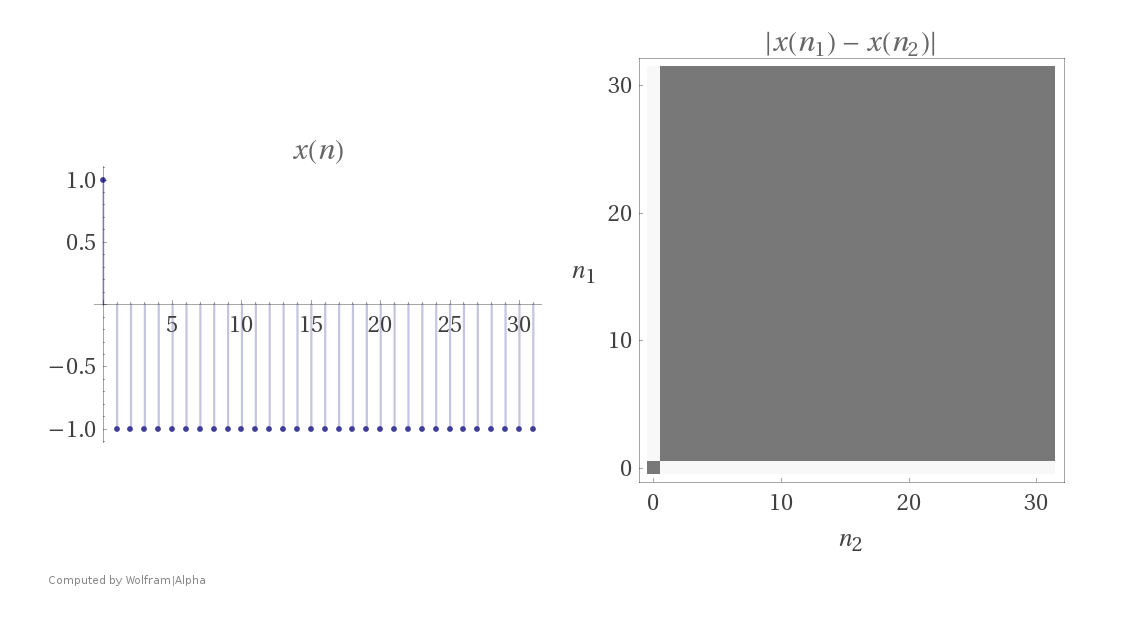
\includegraphics[width=.8\linewidth]{WolfPlots/-2-1}  
		\caption*{Graficzne przedstawienie $x_{0}=-1$ i $c = -2$ }
		
	\end{subfigure}
\end{figure}\\
\begin{figure}[ht]
	\centering
	\begin{subfigure}{1\textwidth}
		\centering
		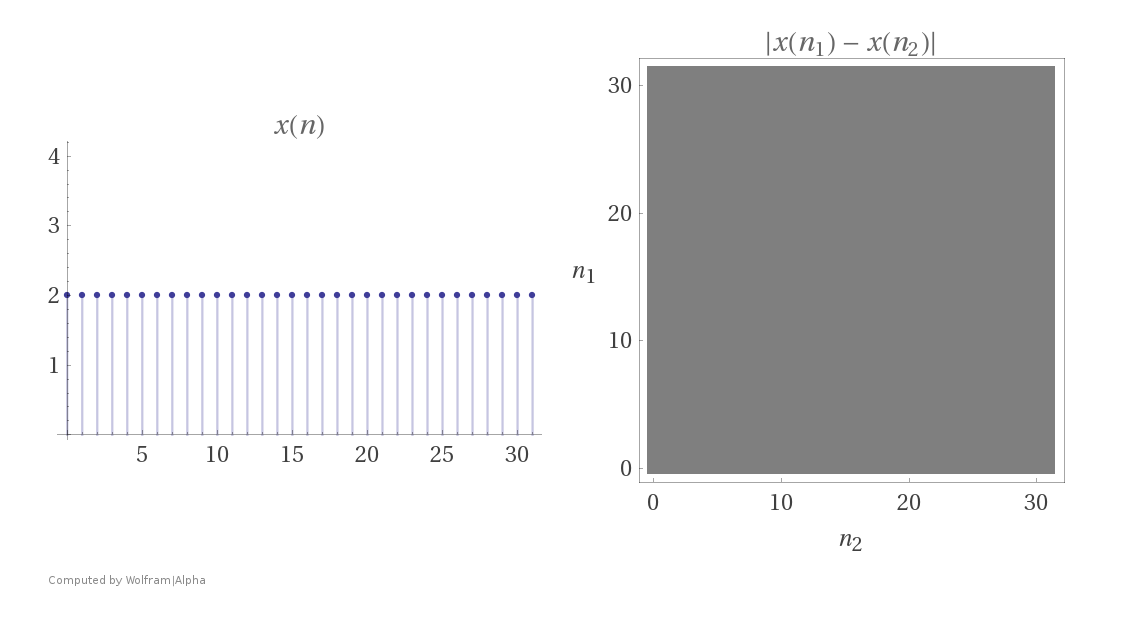
\includegraphics[width=.8\linewidth]{WolfPlots/-2-2}  
		\caption*{Graficzne przedstawienie $x_{0}=2$ i $c = -2$ }
		
	\end{subfigure}
\end{figure}\\
\begin{figure}[ht]
\centering
\begin{subfigure}{1\textwidth}
	\centering
	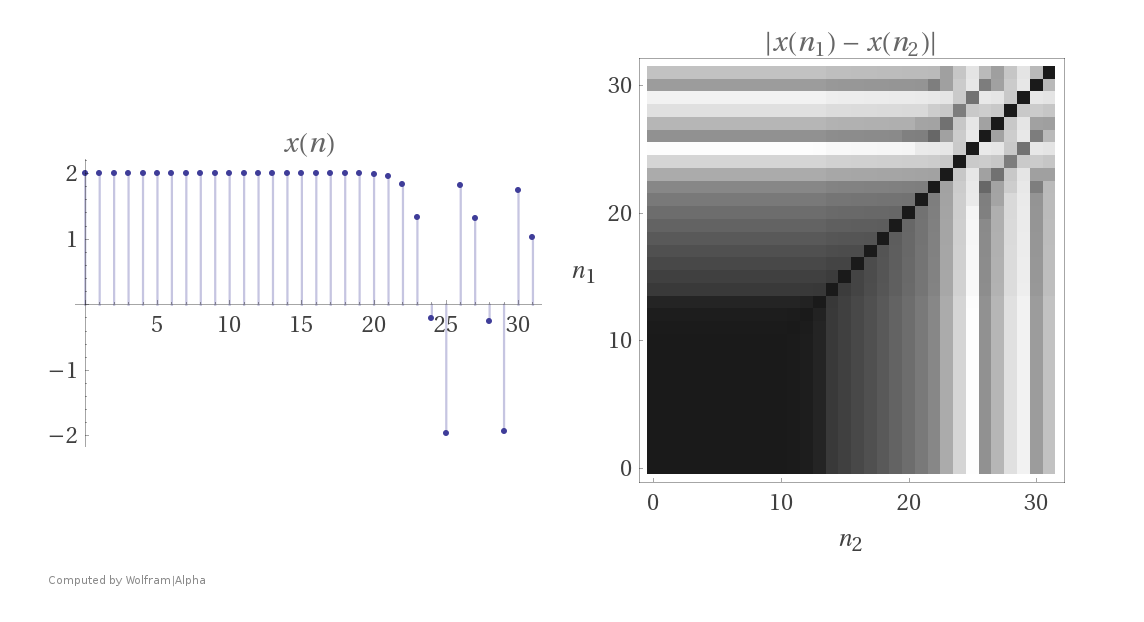
\includegraphics[width=.8\linewidth]{WolfPlots/-2-19999999}  
	\caption*{Graficzne przedstawienie $x_{0}=-1.99999999999999$ i $c = -2$ }
	
\end{subfigure}
\end{figure}\\
\begin{figure}[ht]
	\centering
	\begin{subfigure}{1\textwidth}
		\centering
		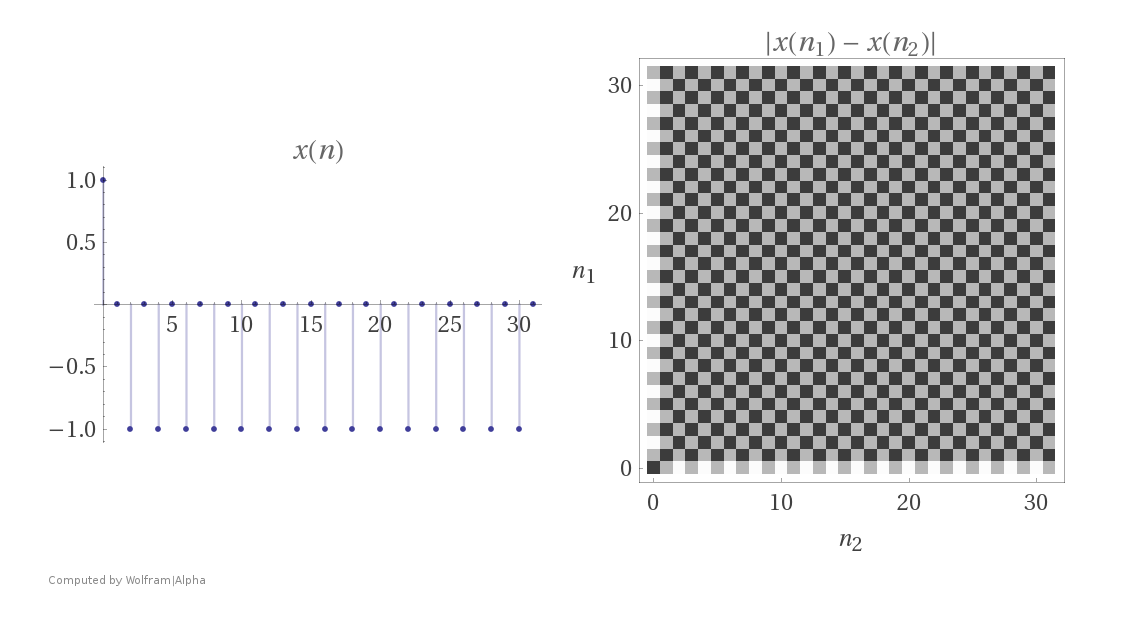
\includegraphics[width=.8\linewidth]{WolfPlots/-1-1}  
		\caption*{Graficzne przedstawienie $x_{0}=1$ i $c = -1$ }
		
	\end{subfigure}
\end{figure}\\
\begin{figure}[ht]
	\centering
	\begin{subfigure}{1\textwidth}
		\centering
		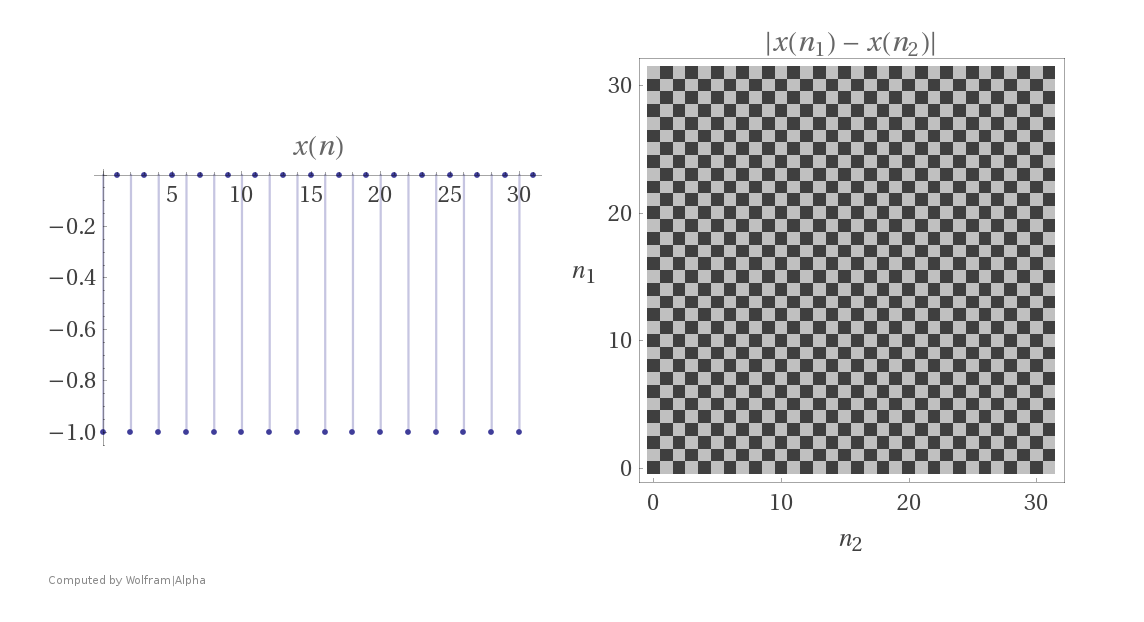
\includegraphics[width=.8\linewidth]{WolfPlots/-1--1}  
		\caption*{Graficzne przedstawienie $x_{0}=-1$ i $c = -1$ }
		
	\end{subfigure}
\end{figure}\\
\begin{figure}[ht]
	\centering
	\begin{subfigure}{1\textwidth}
		\centering
		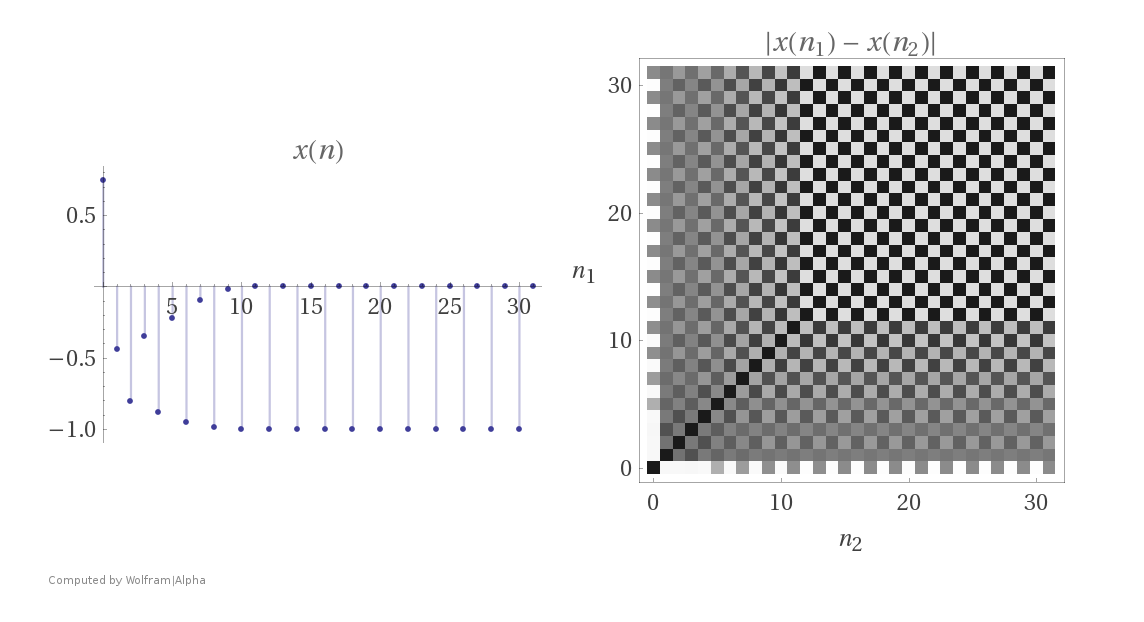
\includegraphics[width=.8\linewidth]{WolfPlots/-1-075}  
		\caption*{Graficzne przedstawienie $x_{0}=0.75$ i $c = -1$ }
		
	\end{subfigure}
\end{figure}\\
\clearpage
\begin{figure}[ht]
	\centering
	\begin{subfigure}{1\textwidth}
		\centering
		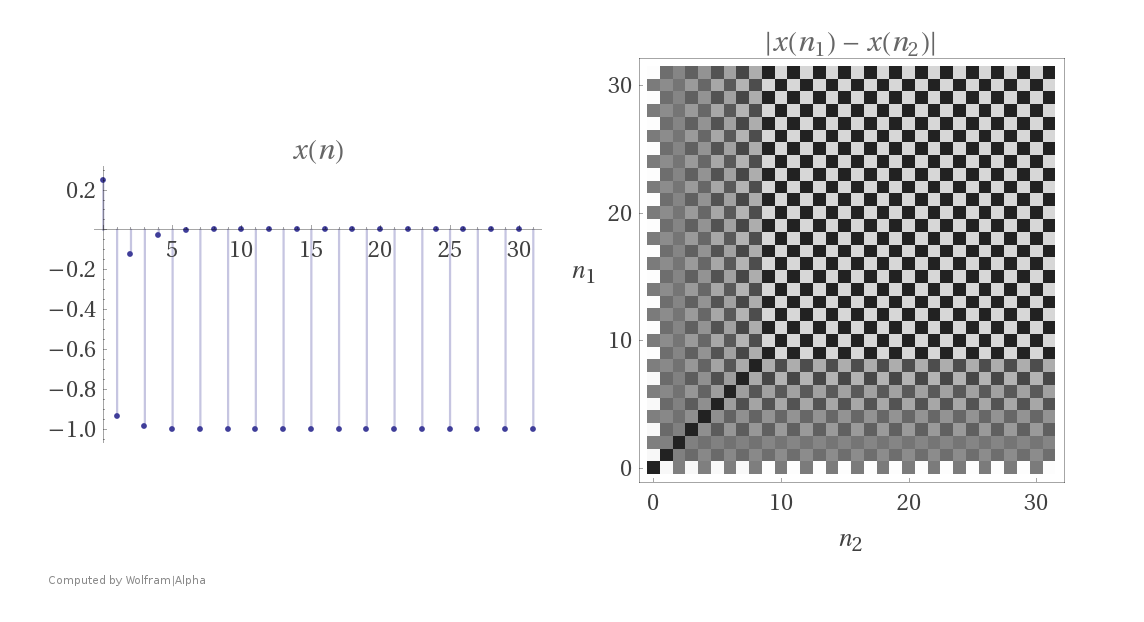
\includegraphics[width=.8\linewidth]{WolfPlots/-1-025}  
		\caption*{Graficzne przedstawienie $x_{0}=0.25$ i $c = -1$ }
		
	\end{subfigure}
\end{figure}
\noindent \textbf{Wnioski:}\\\\
Wykonane przez nas doświadczenie ma związek z pojęciem \textit{układu stabilnego}. Stabilność układu określa to jak pewien układ matematyczny jest wrażliwy na zmiany danych. Dla $x_{0}=-1, c = -2$ oraz 
$x_{0}=2, c = -2$ obserowany układ jest układem stabilnym, otrzymujemy ciągi zbieżne odpowiednio do -1 i 2. Dla $x_{0}=-1.99999999999999, c = -2$ otrzymaliśmy układ niestabliny, od pewnego punktu otrzymane wyniki są losowe. Dla  $c = -1$ każdy zaprezentowany układ jest stabilny, ponieważ mimo początkowej niestabilności, wraz we wzrostem iteracji tworzą się podciągi zbieżne.
\end{document}
